% !TeX program = pdflatex
% !TeX encoding = UTF-8
\documentclass[11pt,aspectratio=169,t]{beamer}
% Все презентации курса компилируются только pdflatex.
\usepackage{iftex}
\RequirePDFTeX
\usepackage{cmap}
\usepackage[T2A]{fontenc}
\usepackage[utf8]{inputenc}
\usepackage[english,russian]{babel}
\usepackage{PTSerif}
\usepackage{amsmath,amsfonts,amssymb}
\usepackage{graphicx,microtype,anyfontsize,tikz}
\usepackage{ragged2e}
\usetikzlibrary{arrows.meta,calc}

\usetheme{default}
\usefonttheme{serif}
\DeclareMathOperator{\sen}{sen}
\bibliographystyle{apalike}

% Общие сведения; номер лекции, её название и дата задаются в N.tex.
\newcommand{\coursename}{Введение в маневрирование КА}
\author{Чиняев Владимир Николаевич}
\institute{Московский физико-технический институт}

% Книжное оформление с голубым акцентом.
\definecolor{coursepaper}{HTML}{FBF9F3}
\definecolor{courseink}{HTML}{302B28}
\definecolor{courseaccent}{HTML}{187AA5}
\definecolor{coursemuted}{HTML}{6D6560}
\definecolor{courserule}{HTML}{A9CADA}
\definecolor{coursetint}{HTML}{EDF4F6}
\tikzset{
  course diagram/.style={font=\fontsize{9.5}{11.5}\selectfont,
    line cap=round,line join=round,>=Latex},
  orbit line/.style={draw=courseaccent,line width=1pt},
  aux line/.style={draw=courserule,line width=.5pt},
  vector line/.style={draw=courseink,line width=.65pt,->},
  angle line/.style={draw=courseaccent,line width=.8pt,->},
  orbit point/.style={circle,fill=courseaccent,inner sep=1.7pt}
}
\setbeamercolor{normal text}{fg=courseink,bg=coursepaper}
\setbeamercolor{background canvas}{bg=coursepaper}
\setbeamercolor{structure}{fg=courseaccent}
\setbeamercolor{alerted text}{fg=courseaccent}
\setbeamercolor{frametitle}{fg=courseink,bg=coursepaper}
\setbeamercolor{footline}{fg=coursemuted,bg=coursepaper}
\setbeamercolor{caption name}{fg=courseaccent}

% Основной текст — 11/14 pt; подписи к рисункам — 9.5/11.5 pt.
\let\coursenormalsize\normalsize
\renewcommand{\normalsize}{\coursenormalsize\fontsize{11}{14}\selectfont}
\setbeamerfont{normal text}{size*={11pt}{14pt}}
\setbeamerfont{frametitle}{size*={20pt}{23pt},series=\mdseries}
\setbeamerfont{title}{size*={27pt}{31pt},series=\mdseries}
\setbeamerfont{subtitle}{size*={12.8pt}{15pt},series=\mdseries}
\setbeamerfont{author}{size*={10.8pt}{13pt}}
\setbeamerfont{institute}{size*={9.2pt}{11pt}}
\setbeamerfont{date}{size*={9pt}{11pt}}
\setbeamerfont{footline}{size*={6.8pt}{8pt}}
\setbeamerfont{caption}{size*={9.5pt}{11.5pt}}
\setbeamerfont{itemize/enumerate body}{size*={11pt}{14pt}}
\setbeamerfont{itemize/enumerate subbody}{size*={11pt}{14pt}}
\setbeamerfont{itemize/enumerate subsubbody}{size*={11pt}{14pt}}
\AtBeginDocument{\normalsize}

\setbeamersize{text margin left=6mm,text margin right=6mm}
\setbeamertemplate{navigation symbols}{}
\setbeamertemplate{headline}{}
\setbeamertemplate{caption}[numbered]
\setbeamertemplate{itemize items}[circle]

% Стандартные блоки Beamer позволяют группировать текст и формулы.
\setbeamertemplate{blocks}[default]
\setbeamerfont{block title}{size*={11pt}{14pt},series=\bfseries}
\setbeamerfont{block body}{size*={11pt}{14pt}}
\setbeamercolor{block title}{fg=courseaccent,bg=coursepaper}
\setbeamercolor{block body}{fg=courseink,bg=coursetint}
\setbeamercolor{block title alerted}{parent=block title}
\setbeamercolor{block body alerted}{parent=block body}
\setbeamercolor{block title example}{parent=block title}
\setbeamercolor{block body example}{parent=block body}

% Компактный заголовок; его высота учитывается при размещении содержания.
\setbeamertemplate{frametitle}{%
  \vskip4.5mm%
  \begin{beamercolorbox}[wd=\textwidth,sep=0pt]{frametitle}
    \usebeamerfont{frametitle}\strut\insertframetitle\strut\par
    \vskip2mm%
    {\color{courseaccent}\hrule height .55pt}
  \end{beamercolorbox}%
}

% Нижний колонтитул: курс слева, лекция и номер слайда справа.
\setbeamertemplate{footline}{%
  \begin{beamercolorbox}[wd=\paperwidth,ht=5.5mm,dp=0pt]{footline}
    \begin{tikzpicture}[remember picture,overlay,x=1mm,y=1mm]
      \begin{scope}[shift={(current page.south west)}]
        \draw[courserule,line width=.3pt] (6,5.5)--(154,5.5);
        \node[text=coursemuted,anchor=west,inner sep=0pt,
          font=\usebeamerfont{footline}] at (6,2.8) {\coursename};
        \node[text=coursemuted,anchor=east,inner sep=0pt,
          font=\usebeamerfont{footline}] at (154,2.8)
          {Лекция \arabic{lecture}\quad\textbullet\quad\insertframenumber};
      \end{scope}
    \end{tikzpicture}%
  \end{beamercolorbox}%
}

% Титульник рассчитан на 16:9 (160 × 90 мм), без нижнего колонтитула.
\setbeamertemplate{title page}{%
  \begin{tikzpicture}[remember picture,overlay,x=1mm,y=1mm]
    \begin{scope}[shift={(current page.south west)}]
      \node[text=coursemuted,anchor=north,font=\usebeamerfont{institute}]
        at (80,82) {\insertinstitute};
      \draw[courseaccent,line width=.55pt] (71,71)--(89,71);
      \node[text=courseink,align=center,text width=125mm,
        font=\usebeamerfont{title}] at (80,53)
        {\hyphenpenalty=10000\coursename\par};
      \node[text=courseaccent,align=center,text width=145mm,font=\usebeamerfont{subtitle}]
        at (80,32) {Лекция \arabic{lecture}. \inserttitle};
      \node[text=courseink,font=\usebeamerfont{author}]
        at (80,19) {\insertauthor};
      \node[text=coursemuted,font=\usebeamerfont{date}]
        at (80,9) {\insertdate};
    \end{scope}
  \end{tikzpicture}%
}

\usepackage{booktabs,array}
\setlength{\abovedisplayskip}{5pt}
\setlength{\belowdisplayskip}{5pt}
\setlength{\abovedisplayshortskip}{3pt}
\setlength{\belowdisplayshortskip}{4pt}
\newcommand{\eqcompact}{\fontsize{10}{12}\selectfont}
\newcommand{\figcaption}[1]{{\usebeamerfont{caption}\color{coursemuted}#1\par}}
\newcommand{\derivationmathspacing}{%
  \setlength{\abovedisplayskip}{2pt}%
  \setlength{\belowdisplayskip}{3pt}%
  \setlength{\abovedisplayshortskip}{2pt}%
  \setlength{\belowdisplayshortskip}{2pt}%
  \setlength{\jot}{2pt}}
\newcommand{\vect}[1]{\boldsymbol{#1}}
\newcommand{\dd}{\mathop{}\!\mathrm d}
\newcommand{\norm}[1]{\left\lVert#1\right\rVert}
\setcounter{lecture}{10}
\title{Задача выведения КА на орбиту}
\date{24 ноября 2026 г.}
% Generated by ascent_numerics.py; units documented in source.
\newcommand{\AscentTOne}{134{,}491}
\newcommand{\AscentRaise}{147{,}286}
\newcommand{\AscentCoast}{301{,}229}
\newcommand{\AscentCircularize}{83{,}044}
\newcommand{\AscentFinalTime}{666{,}050}
\newcommand{\AscentFinalMass}{12{,}245}
\newcommand{\AscentReserve}{3{,}245}
\newcommand{\AscentCharSpeed}{10{,}048}
\newcommand{\AscentGravityLoss}{2303{,}188}
\newcommand{\AscentDragLoss}{36{,}440}
\newcommand{\AscentSteeringLoss}{177{,}407}
\newcommand{\AscentMaxQ}{31{,}508}
\newcommand{\AscentMaxQAlpha}{0{,}723}
\newcommand{\AscentMaxLoad}{6{,}662}
\newcommand{\AscentPositionCheck}{1.20\cdot10^{-7}}
\newcommand{\AscentVelocityCheck}{3.32\cdot10^{-10}}
\newcommand{\AscentEccentricity}{8.28\cdot10^{-14}}
\newcommand{\AscentResidual}{4.66\cdot10^{-14}}
\newcommand{\AscentBalanceError}{-6.22\cdot10^{-12}}


\begin{document}

\begin{frame}[plain]\titlepage\end{frame}

% Постановка и конечная орбита: глава 1 ascent-to-orbit.tex.
\begin{frame}{Постановка задачи выведения}
\relax\derivationmathspacing
\begin{columns}[T,onlytextwidth]
\begin{column}{.49\textwidth}
\textbf{Начальное состояние}
{\eqcompact
\[
\begin{aligned}
 \vect R(t_0)&=\vect R_0,\\
 \vect V(t_0)&=\vect V_0,\\
 m(t_0)&=m_0.
\end{aligned}
\]
}
\textbf{Требуемое конечное состояние}
{\eqcompact
\[
\boxed{\begin{aligned}
 \vect R(t_f)&=\vect R_*,\\
 \vect V(t_f)&=\vect V_*.
\end{aligned}}
\]
}
Пара $\vect R_*,\vect V_*$ соответствует целевой орбите.
При свободной фазе выбирается точка на этой орбите.
\end{column}
\begin{column}{.48\textwidth}
\begin{itemize}
\setlength{\itemsep}{2pt}
 \item $\vect R,\vect V$ --- инерциальные положение и скорость; $m$ --- масса.
 \item Заданы $\mu$, атмосфера, массы ступеней и характеристики двигателей.
 \item Ищутся тяга $F(t)$, её единичное направление $\vect u(t)$ и моменты смены участков.
 \item Проверяются топливо и нагрузки на всём полёте.
 \item $t_f$ может быть задан или определяться программой.
\end{itemize}
\end{column}
\end{columns}
\end{frame}

\begin{frame}{Круговая целевая орбита}
\relax\derivationmathspacing
{\eqcompact
\[
\boxed{r(t_f)=r_*,\qquad V_r(t_f)=0,\qquad
 V_t(t_f)=V_*=\sqrt{\mu/r_*}.}
\]
}
{\centering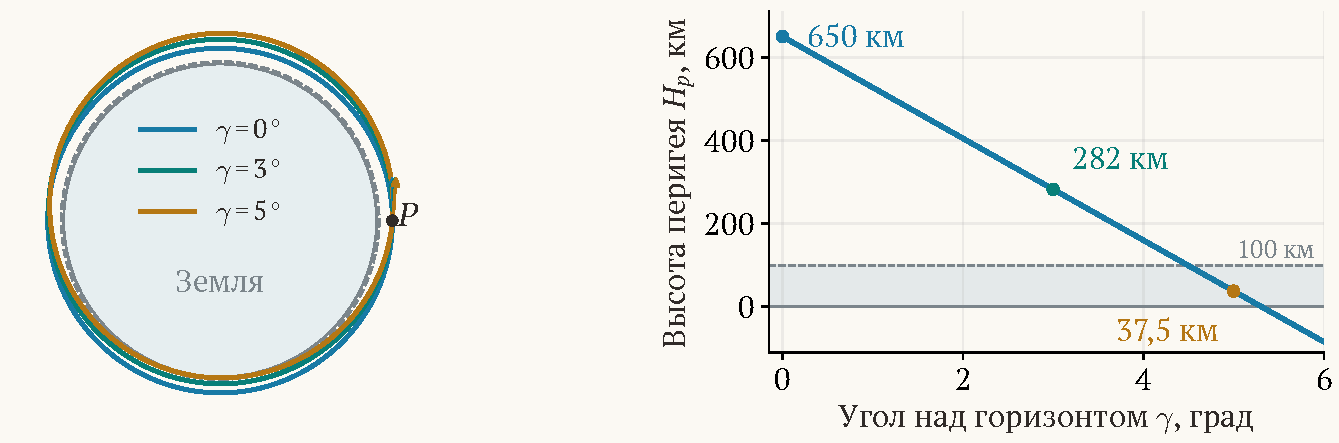
\includegraphics[width=\textwidth,height=42mm,keepaspectratio]{images/geometry-orbits-slide.pdf}\par}
\figcaption{$r=\norm{\vect R}$, $H=r-R_E$; $V_r,V_t$ --- радиальная и трансверсальная скорости.
При одинаковых $H$ и $V$ угол $\gamma$ меняет орбиту: проверяется весь набор конечных условий.}
\end{frame}

% Динамика и масса: глава 2 методички.
\begin{frame}{Уравнения движения}
\relax\derivationmathspacing
\begin{columns}[T,onlytextwidth]
\begin{column}{.49\textwidth}
\textbf{Материальная точка с переменной массой}
{\eqcompact
\[
\begin{aligned}
 \dot{\vect R}&=\vect V,\\[2pt]
 \dot{\vect V}&=-\frac{\mu}{r^3}\vect R
                  +\frac Fm\vect u+\frac{\vect D}{m},\\[2pt]
 \dot m&=-\frac Fc,\qquad r=\norm{\vect R},\\
 c&=g_0I_{\mathrm{sp}},\qquad\norm{\vect u}=1.
\end{aligned}
\]
}
Модель записана в инерциальных координатах.
Подъёмная сила не учитывается.
\end{column}
\begin{column}{.48\textwidth}
\begin{itemize}
\setlength{\itemsep}{3pt}
 \item $F$ --- модуль тяги; $\vect u$ --- её направление.
 \item $\vect D$ --- сила сопротивления атмосферы.
 \item $c$ --- эффективная скорость истечения; $I_{\mathrm{sp}}$ --- удельный импульс.
 \item $g_0$ --- стандартное ускорение.
\end{itemize}
\smallskip
При постоянных $F,c$ масса убывает линейно, а $F/m$ растёт.
При $F=0$ топливо не расходуется.
\end{column}
\end{columns}
\end{frame}

\begin{frame}{Движение относительно воздуха}
\relax\derivationmathspacing
{\eqcompact
\[
 \vect V_{\mathrm{air}}=\vect V-\vect\omega_E\times\vect R-\vect w_{\mathrm{wind}},
 \qquad V_{\mathrm{air}}=\norm{\vect V_{\mathrm{air}}}.
\]
}
\begin{columns}[T,onlytextwidth]
\begin{column}{.49\textwidth}
\textbf{Скоростной напор и сопротивление}
{\eqcompact
\[
 q_{\mathrm{dyn}}=\frac12\rho(H)V_{\mathrm{air}}^2,
 \qquad H=r-R_E,
\]
\[
 D=q_{\mathrm{dyn}}C_DS,
\]
\[
 \vect D=-\frac12\rho(H)C_DS\,
                  V_{\mathrm{air}}\vect V_{\mathrm{air}}.
\]
}
$\rho(H)$ --- плотность; $C_D$ --- коэффициент сопротивления;
$S$ --- опорная площадь.
\end{column}
\begin{column}{.48\textwidth}
\begin{itemize}
\setlength{\itemsep}{3pt}
 \item $\vect\omega_E$ --- угловая скорость вращения Земли.
 \item $\vect\omega_E\times\vect R$ --- линейная скорость вращения атмосферы в точке $\vect R$.
 \item $\vect w_{\mathrm{wind}}$ --- ветер относительно вращающейся Земли.
\end{itemize}
\smallskip
Сопротивление направлено против воздушной скорости.
При $V_{\mathrm{air}}=0$ имеем $\vect D=0$.
\end{column}
\end{columns}
\end{frame}

\begin{frame}{Характеристическая скорость}
\relax\derivationmathspacing
\begin{columns}[T,onlytextwidth]
\begin{column}{.49\textwidth}
\textbf{Интеграл тягового ускорения}
{\eqcompact
\[
 F\dd t=-c\dd m,\qquad c=\mathrm{const},
\]
\[
 \begin{aligned}
 \Delta V_{\mathrm{th}}
 &=\int_{t_b}^{t_e}\frac Fm\dd t
 =-c\int_{m_b}^{m_e}\frac{\dd m}{m}.
 \end{aligned}
\]
\[
 \boxed{\Delta V_{\mathrm{th}}=c\ln\frac{m_b}{m_e}.}
\]
}
$t_b,t_e$ --- начало и конец работы двигателя;
$m_b,m_e$ --- массы в эти моменты.
\end{column}
\begin{column}{.48\textwidth}
\textbf{Длительность при постоянной тяге}
{\eqcompact
\[
 \dot m=-\frac Fc=\mathrm{const},
\]
\[
 \boxed{t_e-t_b=\frac{c(m_b-m_e)}F.}
\]
}
Характеристическая скорость связана с отношением масс.
\par\smallskip
На выведении она отличается от приращения скорости:
действуют сила тяжести и сопротивление,
а тяга может быть отклонена от скорости.
\end{column}
\end{columns}
\end{frame}

\begin{frame}{Разделение ступеней}
\relax\derivationmathspacing
\begin{columns}[T,onlytextwidth]
\begin{column}{.60\textwidth}
\centering
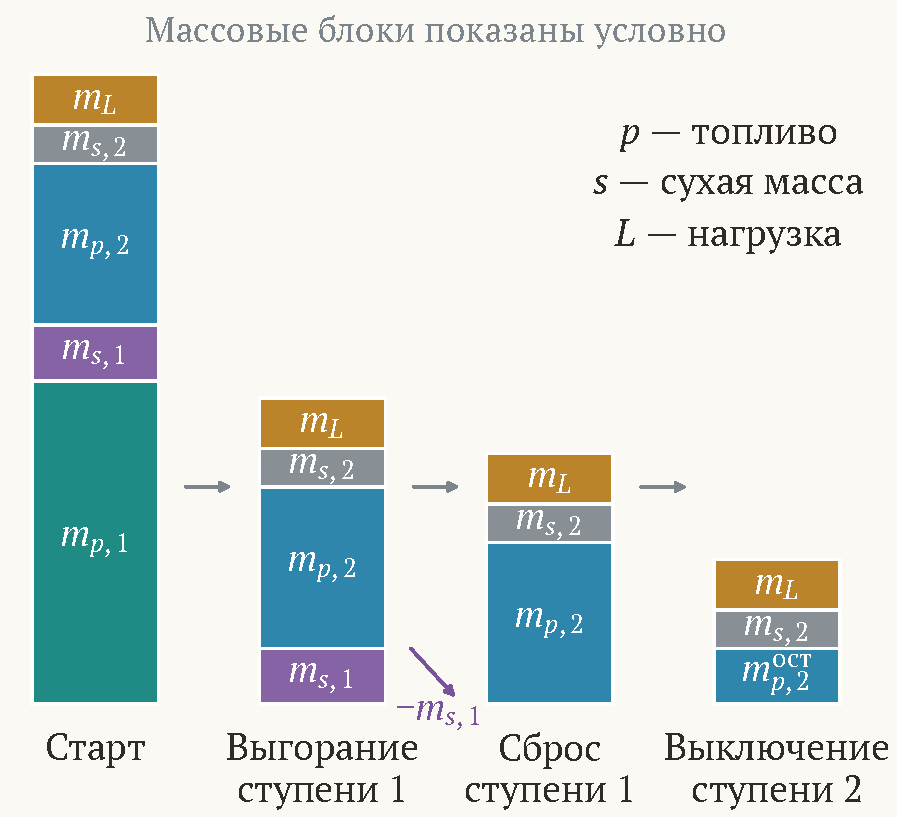
\includegraphics[width=\linewidth,height=55mm,keepaspectratio]{images/geometry-staging-slide.pdf}
\end{column}
\begin{column}{.37\textwidth}
{\eqcompact
\[
 \begin{aligned}
 \vect R^+&=\vect R^-,\\
 \vect V^+&=\vect V^-,\\
 m^+&=m^- -m_{s,1}.
 \end{aligned}
\]
}
$m_{s,1}$ --- сбрасываемая сухая масса; $-,+$ --- состояния до и после разделения.
\par\smallskip
$m_L$ --- нагрузка; $m_{s,1},m_{s,2}$ --- сухие массы;
$m_{p,1},m_{p,2}$ --- топливо. «ост» --- его остаток.
\end{column}
\end{columns}
\smallskip
Положение и скорость непрерывны. Меняются масса и параметры двигателя.
\end{frame}

% Поворот траектории: глава 3 методички.
\begin{frame}{Направления скорости и тяги}
\relax\derivationmathspacing
\begin{columns}[T,onlytextwidth]
\begin{column}{.46\textwidth}
Движение в одной плоскости; Земля не вращается, ветра нет.
{\eqcompact
\[
 \vect V=V(\sin\gamma\,\vect e_r+\cos\gamma\,\vect e_t),
\]
\[
 \vect u=\sin\theta\,\vect e_r+\cos\theta\,\vect e_t,
\]
\[
 V_r=V\sin\gamma,\quad V_t=V\cos\gamma,
 \qquad\beta=\theta-\gamma.
\]
}
\begin{itemize}
\setlength{\itemsep}{2pt}
 \item $\vect e_r,\vect e_t$ --- базис ОСК.
 \item $\gamma,\theta$ --- углы скорости и тяги над горизонтом.
 \item $\varphi$ --- угол положения от $X$ против часовой стрелки.
\end{itemize}
\end{column}
\begin{column}{.51\textwidth}
\centering
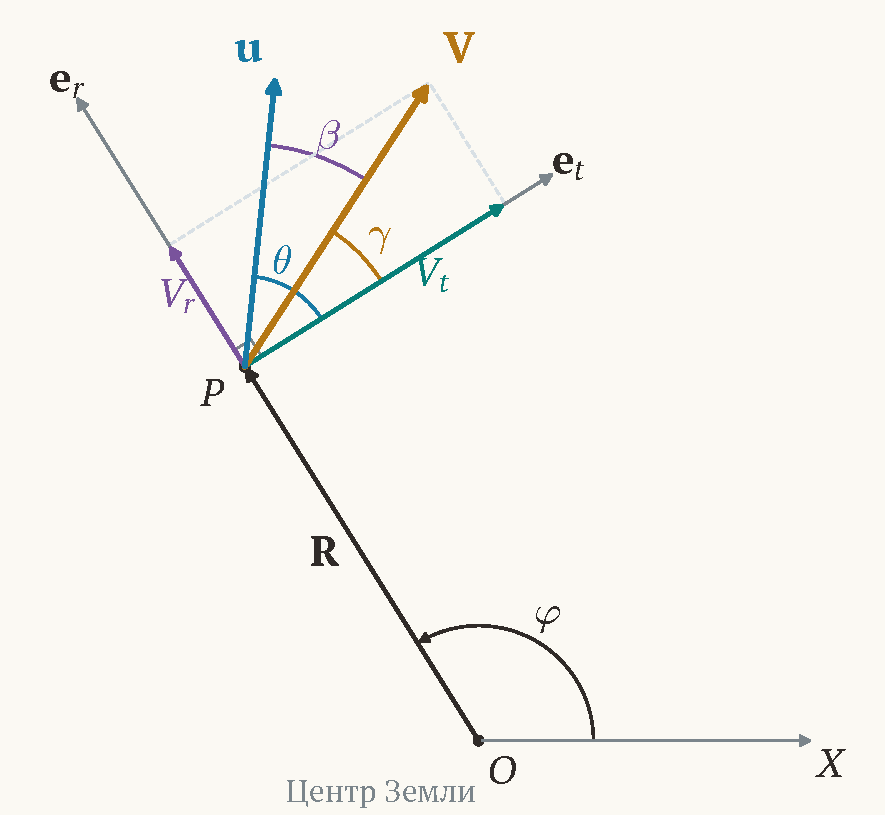
\includegraphics[width=\linewidth,height=59mm,keepaspectratio]{images/geometry-local-frame-slide.pdf}
\end{column}
\end{columns}
\end{frame}

\begin{frame}{Уравнения в естественных переменных}
\relax\derivationmathspacing
\begin{columns}[T,onlytextwidth]
\begin{column}{.48\textwidth}
\textbf{Проекции ускорения}
{\eqcompact
\[
 \dot V=\frac Fm\cos\beta-\frac Dm-g\sin\gamma,
 \qquad g=\frac\mu{r^2},
\]
\[
 V\left(\dot\gamma-\frac{V\cos\gamma}r\right)
 =\frac Fm\sin\beta-g\cos\gamma.
\]
}
Поворот скорости в инерциальных осях отличается от изменения $\gamma$:
местный горизонт также поворачивается со скоростью $V\cos\gamma/r$.
\par\smallskip
Сопротивление направлено вдоль скорости и не входит в нормальную проекцию.
\end{column}
\begin{column}{.49\textwidth}
{\eqcompact
\[
\boxed{\begin{aligned}
 \dot r&=V\sin\gamma,\\
 \dot\varphi&=\pm\frac{V\cos\gamma}r,\\
 \dot V&=\frac Fm\cos\beta-\frac Dm-\frac\mu{r^2}\sin\gamma,\\
 \dot\gamma&=\frac F{mV}\sin\beta
       +\left(\frac Vr-\frac\mu{Vr^2}\right)\cos\gamma,\\
 \dot m&=-\frac Fc.
\end{aligned}}
\]
}
Знак $+$: $\vect e_t$ направлен к росту $\varphi$;
знак $-$: к убыванию, как на предыдущей схеме.
\end{column}
\end{columns}
При $V=0$ угол $\gamma$ не определён: старт рассчитывается в декартовых координатах.
\end{frame}

\begin{frame}{Гравитационный разворот}
\relax\derivationmathspacing
{\eqcompact
\[
 \beta=0:\quad\dot\gamma=\left(\frac Vr-\frac gV\right)\cos\gamma,
 \qquad g=\mu/r^2.
\]
}
{\centering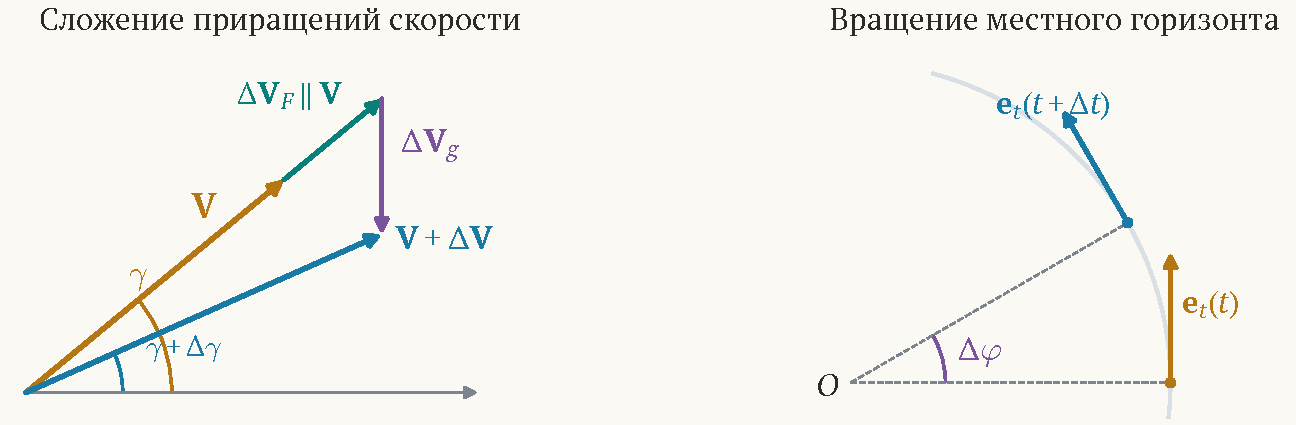
\includegraphics[width=\textwidth,height=37mm,keepaspectratio]{images/geometry-gravity-turn-slide.pdf}\par}
\figcaption{При $\gamma=\pi/2$, $\beta=0$ движение остаётся вертикальным: для выхода из него нужен начальный разворот $\theta<\gamma$.
При $V^2<\mu/r$, $0<\gamma<\pi/2$ угол $\gamma$ уменьшается; при $V^2=\mu/r$ два слагаемых компенсируются.}
\end{frame}

\begin{frame}{Участки программы выведения}
\relax\derivationmathspacing
{\centering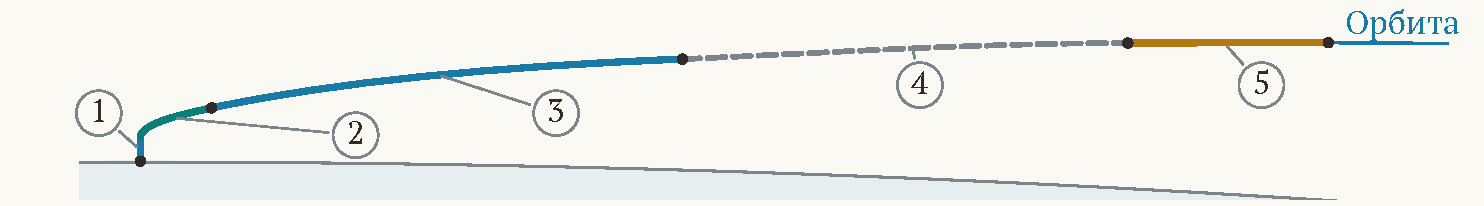
\includegraphics[width=\textwidth,height=26mm,keepaspectratio]{images/geometry-sequence-path-slide.pdf}\par}
\begin{columns}[T,onlytextwidth]
\begin{column}{.49\textwidth}
\begin{enumerate}
\setlength{\itemsep}{2pt}
 \item Вертикальный подъём.
 \item Начальный разворот тяги.
 \item Гравитационный разворот.
\end{enumerate}
\end{column}
\begin{column}{.48\textwidth}
\begin{enumerate}
\setcounter{enumi}{3}
\setlength{\itemsep}{2pt}
 \item Возможная пассивная дуга.
 \item Активное довыведение.
\end{enumerate}
Пассивная пауза нужна не во всех схемах.
\end{column}
\end{columns}
\smallskip
Начальный разворот задаёт исходные условия последующей траектории.
Гравитационный разворот сам по себе не доказывает оптимальность.
\end{frame}

\begin{frame}{Направления на разных участках}
\relax\derivationmathspacing
{\centering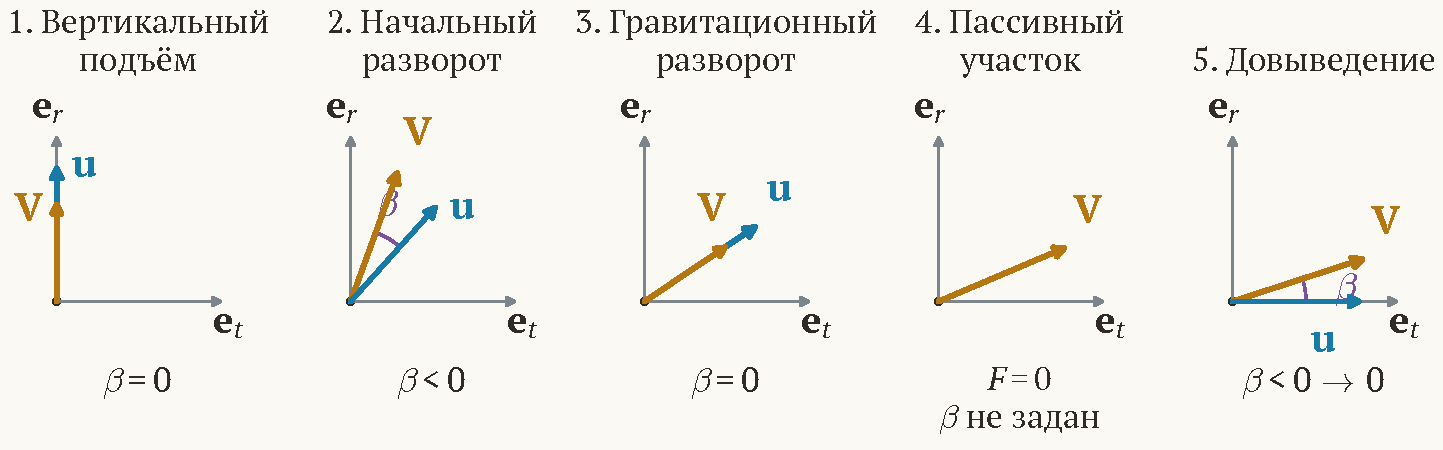
\includegraphics[width=\textwidth,height=45mm,keepaspectratio]{images/geometry-sequence-frames-slide.pdf}\par}
\smallskip
В плотной атмосфере малый угол атаки ограничивает боковые нагрузки.
На пассивном участке $F=0$: направление тяги не задаётся.
Углы на схеме иллюстративные.
\end{frame}

% Потери и ограничения: глава 4 методички.
\begin{frame}{Потери скорости}
\relax\derivationmathspacing
\begin{columns}[T,onlytextwidth]
\begin{column}{.49\textwidth}
{\eqcompact
\[
\begin{aligned}
 \Delta V_{\mathrm{th}}&=\int_{t_0}^{t_f}\frac Fm\dd t,\\
 \Delta V_g&=\int_{t_0}^{t_f}\frac\mu{r^2}\sin\gamma\,\dd t.
\end{aligned}
\]
}
На пассивном подъёме $\Delta V_{\mathrm{th}}$ постоянна,
а $\Delta V_g$ продолжает расти.
\end{column}
\begin{column}{.48\textwidth}
{\eqcompact
\[
\begin{aligned}
 \Delta V_D&=\int_{t_0}^{t_f}\frac Dm\dd t,\\
 \Delta V_{\mathrm{steer}}&=\int_{t_0}^{t_f}\frac Fm(1-\cos\beta)\dd t.
\end{aligned}
\]
}
Крутая траектория быстрее выходит из плотной атмосферы,
но увеличивает $\Delta V_g$.
\end{column}
\end{columns}
{\eqcompact
\[
 \boxed{V_f-V_0=\Delta V_{\mathrm{th}}-\Delta V_g-\Delta V_D-\Delta V_{\mathrm{steer}}.}
\]
}
\figcaption{Использовано $\cos\beta=1-(1-\cos\beta)$.
$V_0,V_f$ --- начальный и конечный модули скорости.
Переход кинетической энергии в потенциальную уже учтён в балансе.}
\end{frame}

\begin{frame}{Напор и нагрузки}
\relax\derivationmathspacing
\begin{columns}[T,onlytextwidth]
\begin{column}{.49\textwidth}
\textbf{Аэродинамические ограничения}
{\eqcompact
\[
 q_{\mathrm{dyn}}=\tfrac12\rho V_{\mathrm{air}}^2\le q_{\max},
\]
\[
 q_{\mathrm{dyn}}|\alpha|\le
       \bigl(q_{\mathrm{dyn}}|\alpha|\bigr)_{\max}.
\]
}
$\alpha$ --- угол оси ракеты к воздушной скорости.
При тяге по оси и невращающейся Земле без ветра $\alpha=\beta$.
\par\smallskip
При ветре или вращении атмосферы направления воздушной и инерциальной скоростей могут различаться.
\end{column}
\begin{column}{.48\textwidth}
\textbf{Единицы и тяговая перегрузка}
Предел произведения задаётся в кПа$\cdot$град или кПа$\cdot$рад.
Угол подставляется в тех же единицах.
\par\smallskip
Переход к радианам: численный предел умножается на $\pi/180$.
{\eqcompact
\[
 \boxed{n_T=\frac F{mg_0}.}
\]
}
При $F=\mathrm{const}$ уменьшение массы увеличивает $n_T$.
В атмосфере продольная нагрузка включает сопротивление.
\end{column}
\end{columns}
\end{frame}

% Пассивная дуга и довыведение: глава 5 методички.
\begin{frame}{Пассивный подъём}
\relax\derivationmathspacing
\begin{columns}[T,onlytextwidth]
\begin{column}{.49\textwidth}
\textbf{Инварианты в вакууме без тяги}
{\eqcompact
\[
 \mathcal E=\frac{V^2}2-\frac\mu r=\mathrm{const},
\]
\[
 \vect h=\vect R\times\vect V=\mathrm{const},
 \qquad h=\norm{\vect h}.
\]
}
Сохраняются большая полуось $a$, эксцентриситет $e$,
радиусы перигея $r_p$ и апогея $r_a$ оскулирующей орбиты.
\par\smallskip
Высота, скорость и угол траектории меняются.
\end{column}
\begin{column}{.48\textwidth}
\textbf{Обмен кинетической и потенциальной энергией}
{\eqcompact
\[
 \boxed{V_2^2=V_1^2+2\mu\left(\frac1{r_2}-\frac1{r_1}\right).}
\]
}
$r_1,r_2$ --- два радиуса на пассивной дуге;
$V_1,V_2$ --- модули скорости в этих положениях.
\par\smallskip
При подъёме скорость уменьшается. В апогее $V_r=0$,
но $V_t$ может оставаться ниже круговой.
\par\smallskip
Если апогей ниже цели, ожиданием нужной высоты достичь нельзя.
\end{column}
\end{columns}
\end{frame}

\begin{frame}{Довыведение в апогее}
\relax\derivationmathspacing
\begin{columns}[T,onlytextwidth]
\begin{column}{.55\textwidth}
\centering
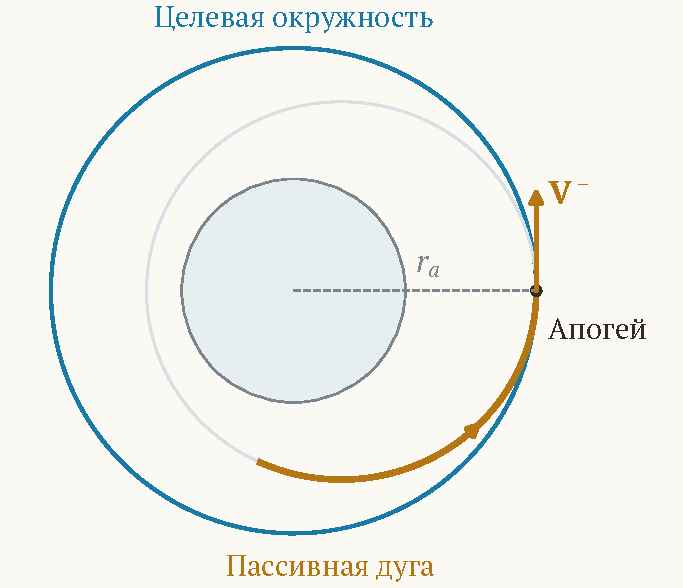
\includegraphics[width=\linewidth,height=56mm,keepaspectratio]{images/geometry-coast-orbit-slide.pdf}
\end{column}
\begin{column}{.42\textwidth}
Промежуточная орбита: $r_a=r_*$.
{\eqcompact
\[
 a_{\mathrm{tr}}=\frac{r_p+r_*}2,
\]
\[
 V_a^-=\sqrt{\mu\left(\frac2{r_*}-\frac1{a_{\mathrm{tr}}}\right)},
\]
\[
 \boxed{\Delta V_{\mathrm{circ}}=\sqrt{\frac\mu{r_*}}-V_a^-.}
\]
}
Трансверсальный импульс поднимает перигей до $r_*$.
\par\smallskip
$V_a^-$ --- скорость перед импульсом.
На схеме --- пассивная дуга.
\end{column}
\end{columns}
\end{frame}

\begin{frame}{Начало активного довыведения}
\relax\derivationmathspacing
{\eqcompact
\[
 r(t_f)=r_*,\qquad V_r(t_f)=0,\qquad V_t(t_f)=\sqrt{\mu/r_*}.
\]
}
\begin{columns}[T,onlytextwidth]
\begin{column}{.49\textwidth}
\textbf{Конечная тяга}
\par\smallskip
За время манёвра меняются положение и скорость.
Начало в точке идеального импульса в общем случае
не обеспечивает круговую орбиту.
\par\smallskip
Начальная $V_r$ может быть положительной.
Сила тяжести и радиальная проекция тяги должны довести её до нуля
за время набора $V_t$.
\end{column}
\begin{column}{.48\textwidth}
\textbf{Пауза и последующий манёвр}
\par\smallskip
Длительность пассивного подъёма определяет,
с какими $r,V_r,V_t$ начинается довыведение.
\par\smallskip
Её подбирают вместе с длительностью
и направлением последнего активного участка.
\end{column}
\end{columns}
\end{frame}

% Пристрелка: глава 6 методички.
\begin{frame}{Конечная невязка}
\relax\derivationmathspacing
\begin{columns}[T,onlytextwidth]
\begin{column}{.49\textwidth}
\textbf{Безразмерная конечная невязка}
{\eqcompact
\[
 \vect{\mathcal R}(\vect p)=
 \begin{pmatrix}
 (r_f-r_*)/r_*\\
 V_{r,f}/V_*\\
 (V_{t,f}-V_*)/V_*
 \end{pmatrix},\qquad
 \norm{\vect{\mathcal R}}_2\le\varepsilon.
\]
}
$\vect p$ --- параметры активных участков и пауз;
$\varepsilon$ --- допуск на евклидову норму.
\par\smallskip
Если $t_f$ свободно, длительность манёвра может входить в $\vect p$.
\end{column}
\begin{column}{.48\textwidth}
\begin{itemize}
\setlength{\itemsep}{4pt}
 \item $r_f,V_{r,f},V_{t,f}$ --- рассчитанные значения в момент $t_f$.
 \item $r_*,V_*$ --- целевые значения и масштабы нормировки.
 \item Все компоненты невязки безразмерны.
 \item Каждая оценка невязки требует прогноза от старта до конца программы.
\end{itemize}
\end{column}
\end{columns}
\smallskip
Пристрелка обеспечивает конечные условия. Максимум остатка топлива требует отдельной оптимизации.
\end{frame}

\begin{frame}{Ньютоновское уточнение}
\relax\derivationmathspacing
\begin{columns}[T,onlytextwidth]
\begin{column}{.49\textwidth}
\textbf{Поправка параметров программы}
{\eqcompact
\[
 \frac{\partial\vect{\mathcal R}}{\partial\vect p}\,
       \delta\vect p=-\vect{\mathcal R}(\vect p),
\]
\[
 \vect p_{\mathrm{new}}=\vect p+\eta\,\delta\vect p,
 \qquad 0<\eta\le1.
\]
}
$\delta\vect p$ --- поправка; $\eta$ --- уменьшение шага.
При $\eta=1$ принимается полный ньютоновский шаг.
\par\smallskip
Производные вычисляются центральными разностями с повторными прогнозами.
\end{column}
\begin{column}{.48\textwidth}
\begin{enumerate}
\setlength{\itemsep}{3pt}
 \item Выполнить прогноз всей траектории.
 \item Найти текущую матрицу производных и поправку.
 \item Проверить новую программу; уменьшить шаг при росте невязки или нарушении ограничений.
 \item Повторять до допуска, затем проверить нагрузки и запас топлива.
\end{enumerate}
\end{column}
\end{columns}
\end{frame}

% Вращение Земли и плоскость запуска: глава 7 методички.
\begin{frame}{Начальная инерциальная скорость}
\relax\derivationmathspacing
\begin{columns}[T,onlytextwidth]
\begin{column}{.53\textwidth}
\centering
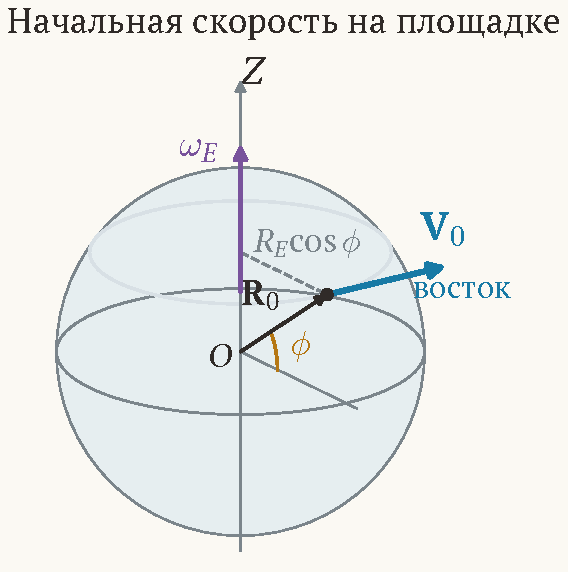
\includegraphics[width=\linewidth,height=59mm,keepaspectratio]{images/geometry-rotation-pad-slide.pdf}
\end{column}
\begin{column}{.44\textwidth}
Ракета на площадке вращается вместе с Землёй.
{\eqcompact
\[
 \vect\omega_E=\omega_E\vect k,
\]
\[
 \vect V_0=\vect\omega_E\times\vect R_0
 =\omega_E R_E\cos\phi\,\vect e_E,
\]
\[
 \boxed{V_{E,0}=\norm{\vect V_0}=\omega_E R_E\cos\phi.}
\]
}
$\phi$ --- широта космодрома; $\vect k$ --- единичный вектор оси $Z$;
$\vect e_E$ --- местный восток.
\par\smallskip
Плечо вращения равно $R_E\cos\phi$.
Других составляющих скорости площадки нет;
на экваторе --- около $465$ м/с.
\end{column}
\end{columns}
\end{frame}

\begin{frame}{Инерциальная и воздушная скорости}
\relax\derivationmathspacing
\begin{columns}[T,onlytextwidth]
\begin{column}{.54\textwidth}
\centering
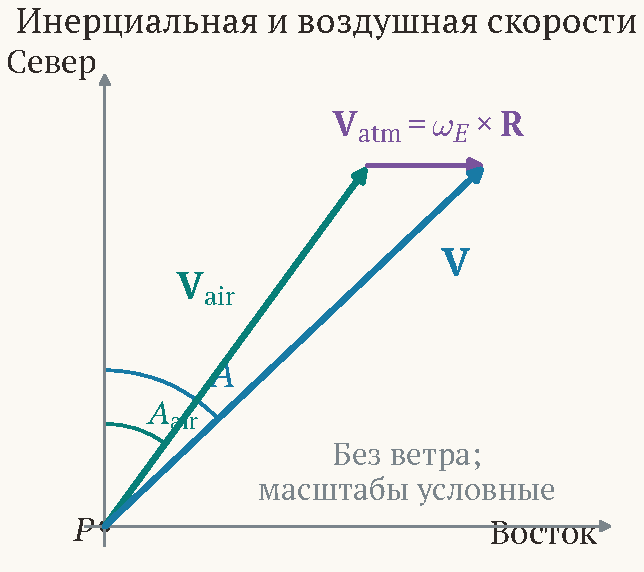
\includegraphics[width=\linewidth,height=58mm,keepaspectratio]{images/geometry-rotation-air-slide.pdf}
\end{column}
\begin{column}{.43\textwidth}
\textbf{Атмосфера без ветра}
{\eqcompact
\[
 \vect V_{\mathrm{atm}}=\vect\omega_E\times\vect R,
\]
\[
 \vect V_{\mathrm{air}}=\vect V-\vect V_{\mathrm{atm}}.
\]
}
Орбиту определяет инерциальная скорость,
а аэродинамику --- скорость относительно воздуха.
\par\smallskip
$A,A_{\mathrm{air}}$ --- их азимуты от севера к востоку.
Различаются и азимуты, и модули скоростей.
\par\smallskip
При ветре дополнительно вычитается $\vect w_{\mathrm{wind}}$.
\end{column}
\end{columns}
\end{frame}

\begin{frame}{Земная ось и местный базис}
\relax\derivationmathspacing
\begin{columns}[T,onlytextwidth]
\begin{column}{.53\textwidth}
\centering
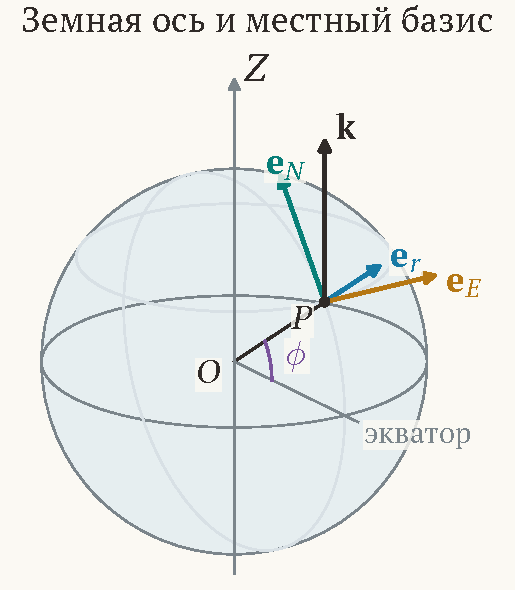
\includegraphics[width=\linewidth,height=59mm,keepaspectratio]{images/geometry-launch-plane-earth-slide.pdf}
\end{column}
\begin{column}{.44\textwidth}
\begin{itemize}
\setlength{\itemsep}{3pt}
 \item $\vect e_r$ --- радиальный вектор.
 \item $\vect e_N,\vect e_E$ --- местные север и восток.
 \item $\vect k$ параллелен оси вращения $Z$.
 \item $\vect e_N$ направлен по касательной к поверхности на север.
\end{itemize}
{\eqcompact
\[
 \boxed{\vect k=\sin\phi\,\vect e_r+\cos\phi\,\vect e_N.}
\]
}
Азимут $A$ отсчитывается от севера к востоку:
$0$ --- север, $90^\circ$ --- восток.
\par\smallskip
$\vect e_A$ --- единичное горизонтальное направление движения.
\end{column}
\end{columns}
\end{frame}

\begin{frame}{Азимут и наклонение}
\relax\derivationmathspacing
\begin{columns}[T,onlytextwidth]
\begin{column}{.53\textwidth}
\centering
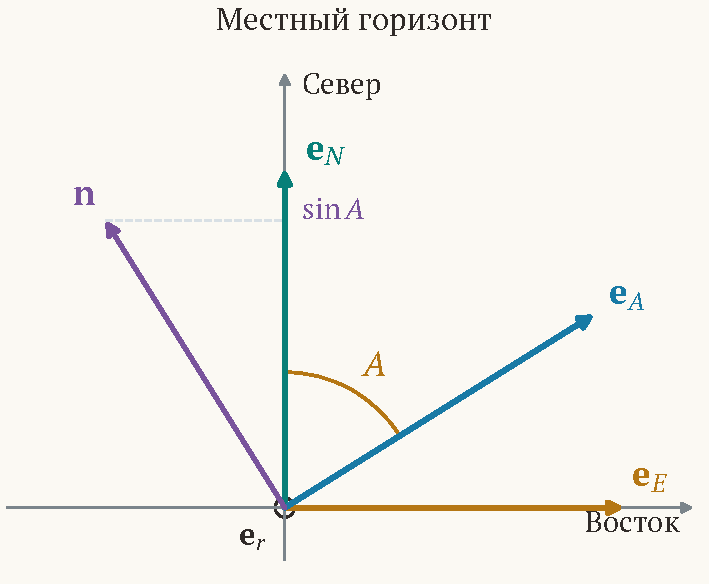
\includegraphics[width=\linewidth,height=57mm,keepaspectratio]{images/geometry-launch-plane-local-slide.pdf}
\end{column}
\begin{column}{.44\textwidth}
Радиальная скорость не вносит вклада в орбитальный момент.
Единичная нормаль орбиты:
{\eqcompact
\[
 \vect n=\frac{\vect R\times\vect V}{\norm{\vect R\times\vect V}}
 =\sin A\,\vect e_N-\cos A\,\vect e_E.
\]
\[
 \boxed{\cos i=\vect n\cdot\vect k=\cos\phi\sin A.}
\]
}
$i$ --- угол между $\vect n$ и $\vect k$;
$A$ --- инерциальный азимут.
\par\smallskip
Широта космодрома даёт исходную оценку
для плоскости, проходящей через него.
\end{column}
\end{columns}
\end{frame}

\begin{frame}{Целевая плоскость и космодром}
\relax\derivationmathspacing
\begin{columns}[T,onlytextwidth]
\begin{column}{.53\textwidth}
\centering
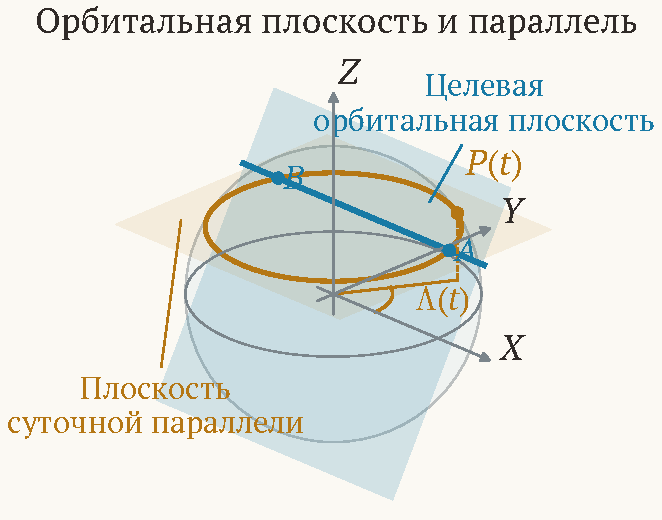
\includegraphics[width=\linewidth,height=59mm,keepaspectratio]{images/geometry-launch-window-plane-slide.pdf}
\end{column}
\begin{column}{.44\textwidth}
При одинаковом наклонении $i$ возможны разные долготы восходящего узла $\Omega$.
\par\smallskip
Для прямого запуска космодром должен попасть
в фиксированную инерциальную плоскость:
{\eqcompact
\[
 \boxed{\vect n_*\cdot\vect R_s(t_0)=0.}
\]
}
$\vect n_*$ --- её единичная нормаль;
$\vect R_s(t)$ --- радиус-вектор космодрома $P(t)$.
\par\smallskip
Синяя линия --- пересечение целевой плоскости с плоскостью суточной параллели.
\end{column}
\end{columns}
\end{frame}

\begin{frame}{Время старта}
\relax\derivationmathspacing
\begin{columns}[T,onlytextwidth]
\begin{column}{.53\textwidth}
\centering
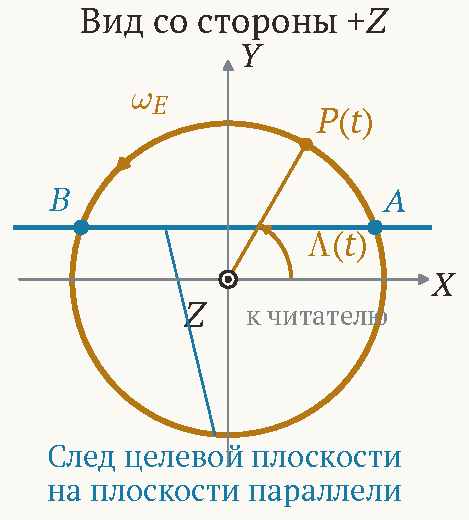
\includegraphics[width=\linewidth,height=59mm,keepaspectratio]{images/geometry-launch-window-top-slide.pdf}
\end{column}
\begin{column}{.44\textwidth}
Инерциальная долгота космодрома $\Lambda(t)$ отсчитывается от $X$ вокруг оси $Z$.
{\eqcompact
\[
 \Lambda(t)=\Lambda_0+\omega_Et,
 \qquad\Lambda_0=\Lambda(0).
\]
}
Точки $A,B$ --- пересечения суточной параллели со следом целевой плоскости.
\par\smallskip
Это геометрическая оценка времени старта.
Полная программа должна учитывать вращение Земли
и движение ракеты за время полёта.
\end{column}
\end{columns}
\end{frame}

% Расчётный пример: глава 8 методички ascent-to-orbit.tex.
\begin{frame}{Учебная двухступенчатая ракета}
\relax\derivationmathspacing
\begin{columns}[T,onlytextwidth]
\begin{column}{.51\textwidth}
{\eqcompact
\centering
\renewcommand{\arraystretch}{1.14}
\setlength{\tabcolsep}{5pt}
\begin{tabular}{@{}lrr@{}}
\toprule
Параметр & 1-я & Верхняя\\\midrule
Топливо, т & $160$ & $45$\\
Сухая масса, т & $16$ & $4$\\
Тяга, МН & $3{,}5$ & $0{,}8$\\
Удельный импульс, с & $300$ & $450$\\
\bottomrule
\end{tabular}\par
}
\smallskip
Нагрузка $5$ т; начальная масса $230$ т.
Тяга и удельный импульс постоянны на каждом активном участке.
\end{column}
\begin{column}{.46\textwidth}
\textbf{Начальное состояние и цель}
{\eqcompact\derivationmathspacing
\[
\vect R_0=(R_E,0)^\top,\qquad \vect V_0=0,
\]
\[
 \begin{gathered}
 r_*=7028{,}137\ \text{км},\\
 V_*=7{,}5309329\ \text{км/с}.
 \end{gathered}
\]
}
Плоская модель сферической Земли без вращения и подъёмной силы.
Атмосфера неподвижна; цель --- круговая орбита $650$ км.
\end{column}
\end{columns}
{\eqcompact\derivationmathspacing
\[
 \mu=398600{,}4418\ \text{км}^3/\text{с}^2,\quad
 R_E=6378{,}137\ \text{км},\quad g_0=9{,}80665\ \text{м/с}^2,
\]
\[
 \rho(H)=1{,}225\exp\!\left(-\frac H{7{,}2\ \text{км}}\right)
 \ \text{кг/м}^3,\qquad C_D=0{,}3,\quad S=10\ \text{м}^2.
\]
}
\end{frame}

\begin{frame}{Программа выведения}
\relax\derivationmathspacing
\begin{columns}[T,onlytextwidth]
\begin{column}{.48\textwidth}
\textbf{Первая ступень}
\begin{enumerate}
\setlength{\itemsep}{4pt}
\item Вертикальная тяга в течение $10$ с.
\item Линейное уменьшение $\theta$ от $90^\circ$ до $70^\circ$ за $25$ с.
\item Тяга вдоль скорости, $\theta=\gamma$, до выгорания топлива.
\end{enumerate}
\smallskip
Время работы $\AscentTOne$ с; масса перед разделением $70$ т, после него $54$ т.
\end{column}
\begin{column}{.49\textwidth}
\textbf{Верхняя ступень}
\begin{enumerate}
\setcounter{enumi}{3}
\setlength{\itemsep}{4pt}
\item Активный участок при $\theta=45^\circ$ формирует переходную дугу.
\item Пассивный подъём при $F=0$.
\item Трансверсальное довыведение, $\theta=0$, до круговой скорости и $V_r=0$.
\end{enumerate}
\smallskip
Двигатель допускает выключение и повторный запуск.
\end{column}
\end{columns}
\smallskip
\justifying
Повороты и переключения идеализированы мгновенными; положение и скорость непрерывны.
Переходные процессы двигателя и корпуса не моделируются.
\end{frame}

\begin{frame}{Траектория выведения}
\relax\derivationmathspacing
{\centering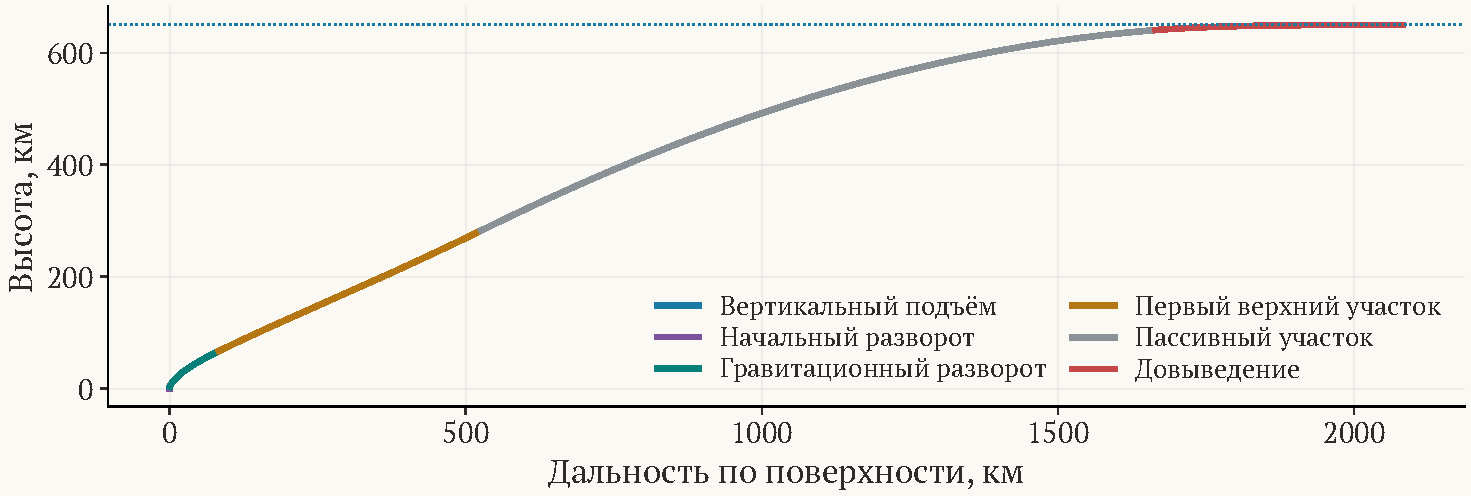
\includegraphics[width=\textwidth,height=46mm,keepaspectratio]{images/ascent-trajectory-slide.pdf}\par}
\justifying
Дальность равна $R_E\varphi$: в примере $\varphi$ отсчитывается от радиуса старта против часовой стрелки в сторону движения.
Масштабы высоты и дальности различны.
\end{frame}

\begin{frame}{Пристрелка длительностей}
\relax\derivationmathspacing
\begin{columns}[T,onlytextwidth]
\begin{column}{.53\textwidth}
{\centering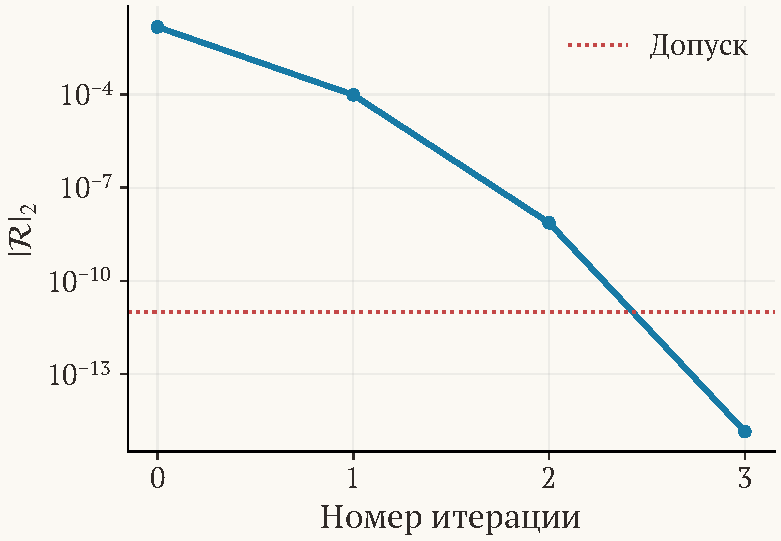
\includegraphics[width=\linewidth,height=44mm,keepaspectratio]{images/ascent-convergence-slide.pdf}\par}
\justifying
Три ньютоновские поправки; полный прогноз от старта.
В расчёте используются полные значения параметров.
\end{column}
\begin{column}{.44\textwidth}
Длительности: $\tau_{\mathrm a}$ --- первого активного участка верхней ступени;
$\tau_{\mathrm c}$ --- пассивной паузы; $\tau_{\mathrm d}$ --- довыведения.
{\eqcompact\derivationmathspacing
\[
 \vect p=(\tau_{\mathrm a},\tau_{\mathrm c},\tau_{\mathrm d})^\top,
\]
\[
 \vect p^{(0)}=(150,300,80)^\top\ \text{с},
\]
\[
 \begin{aligned}
 \tau_{\mathrm a}&=\AscentRaise\ \text{с},\\
 \tau_{\mathrm c}&=\AscentCoast\ \text{с},\\
 \tau_{\mathrm d}&=\AscentCircularize\ \text{с}.
 \end{aligned}
\]
\[
 \tau_{\mathrm a}+\tau_{\mathrm d}\le248{,}231\ \text{с},
 \qquad\norm{\vect{\mathcal R}}_2<10^{-11}.
\]
}
$t_f=\AscentFinalTime$ с; приведённые параметры округлены.
\end{column}
\end{columns}
\end{frame}

\begin{frame}{Высота и компоненты скорости}
\relax\derivationmathspacing
{\centering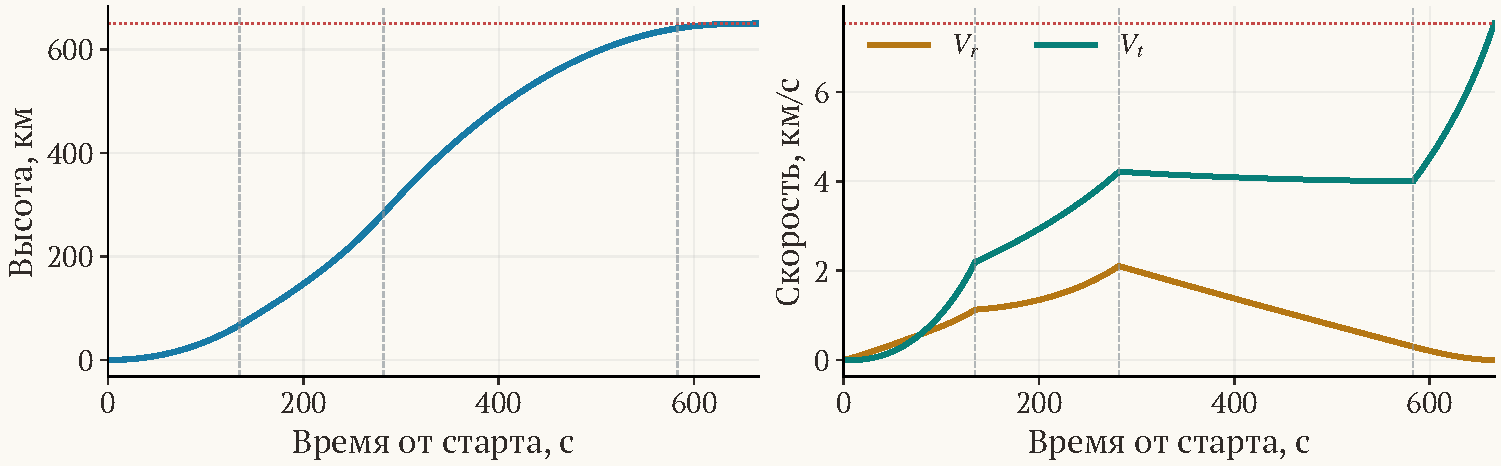
\includegraphics[width=\textwidth,height=44mm,keepaspectratio]{images/ascent-height-speed-slide.pdf}\par}
\justifying
После первого активного участка верхней ступени: высота около $283$ км, $V_r=2{,}10$ км/с.
На пассивной дуге ракета поднимается за счёт уменьшения кинетической энергии.
\end{frame}

\begin{frame}{Углы скорости и тяги}
\relax\derivationmathspacing
{\centering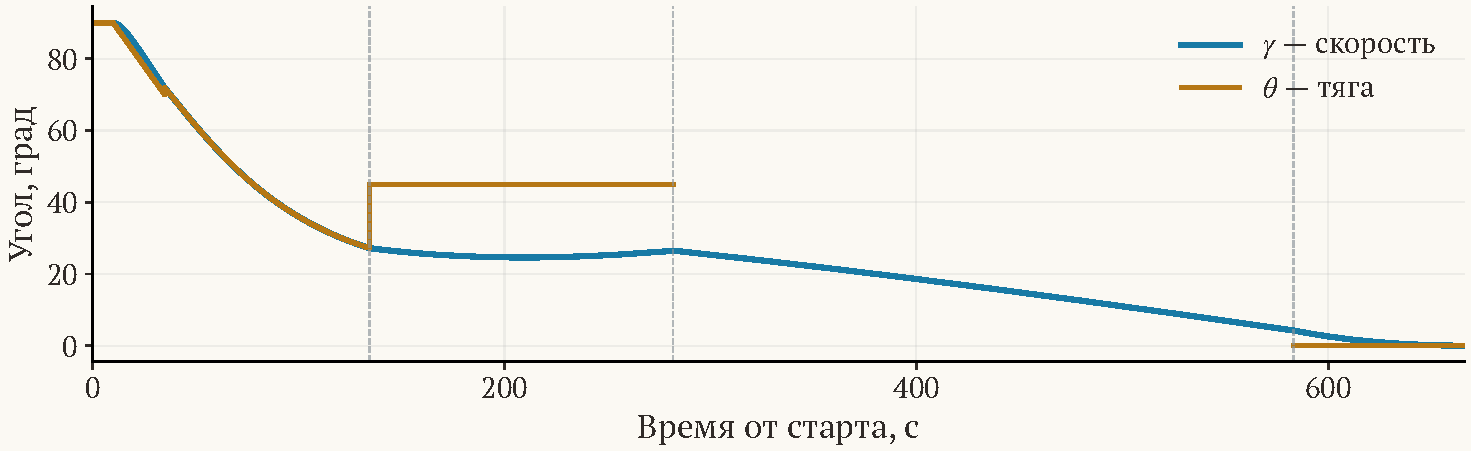
\includegraphics[width=\textwidth,height=44mm,keepaspectratio]{images/ascent-angles-slide.pdf}\par}
\justifying
На гравитационном развороте $\theta=\gamma$; при довыведении $\theta=0$.
На пассивном участке направление тяги не задаётся.
При $V=0$ угол $\gamma$ не определён; $90^\circ$ обозначает вертикальный предел.
\end{frame}

\begin{frame}{Активное довыведение}
\relax\derivationmathspacing
{\centering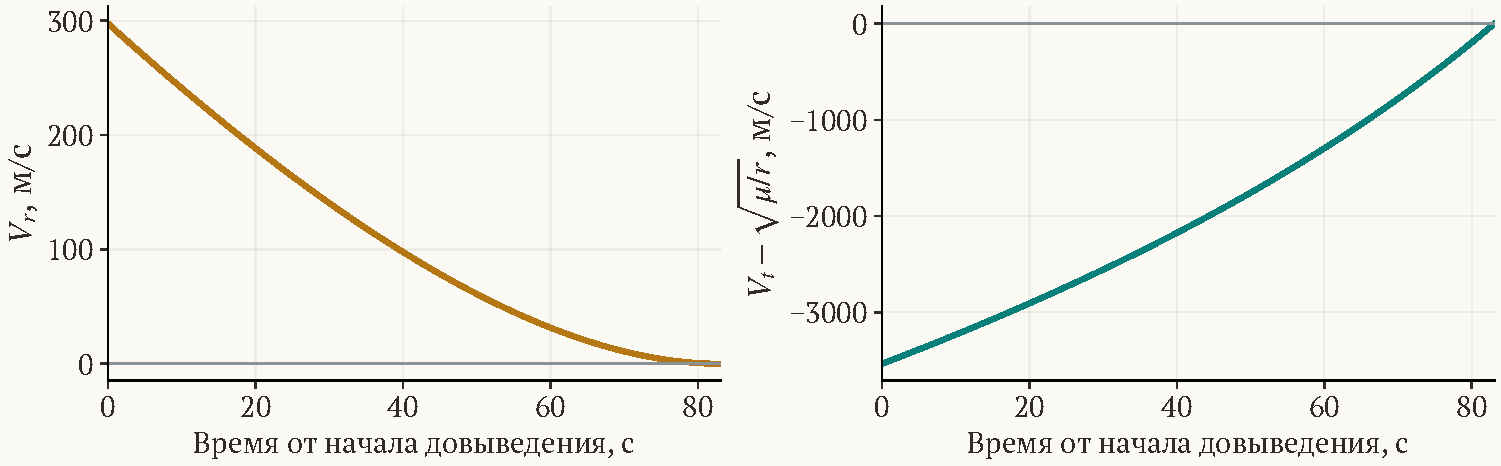
\includegraphics[width=\textwidth,height=36mm,keepaspectratio]{images/ascent-final-insertion-slide.pdf}\par}
{\eqcompact\derivationmathspacing
\[
 H=640{,}845\ \text{км},\quad V_r=0{,}2973\ \text{км/с},\quad
 V_t=3{,}9991\ \text{км/с},\qquad
 \dot V_r=\frac{V_t^2}{r}-\frac\mu{r^2}<0.
\]
}
\justifying
Довыведение начинается до апогея. При трансверсальной тяге и пренебрежимо
малом сопротивлении $V_r$ уменьшается без тяги вниз, пока $V_t<\sqrt{\mu/r}$.
Пауза согласует $V_r=0$ и круговую скорость.
\end{frame}

\begin{frame}{Формирование круговой орбиты}
\relax\derivationmathspacing
{\centering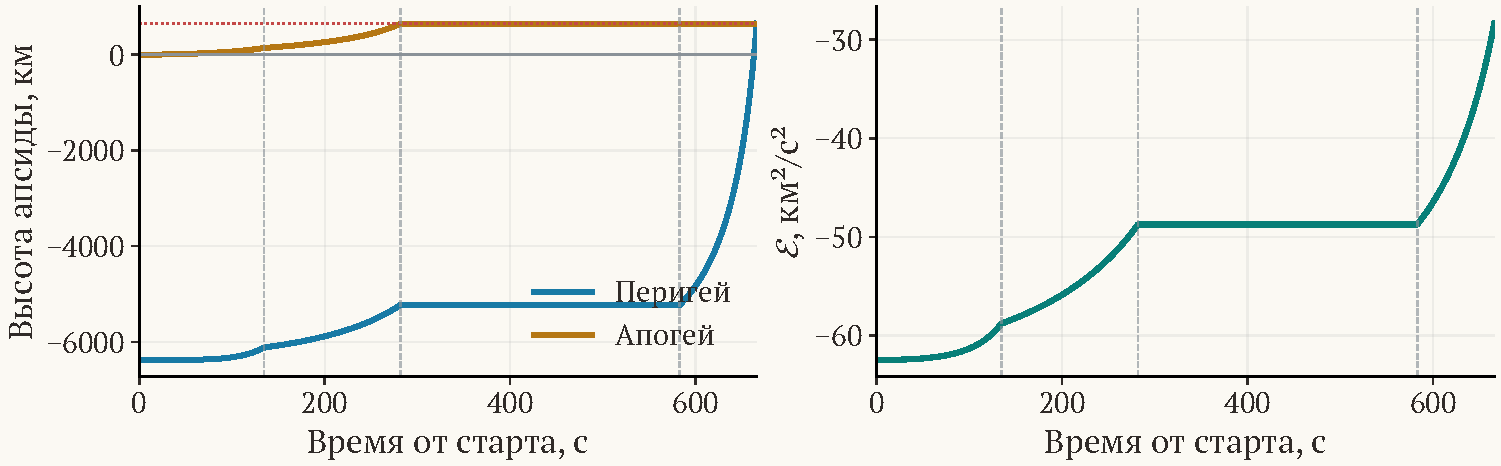
\includegraphics[width=\textwidth,height=44mm,keepaspectratio]{images/ascent-osculating-orbit-slide.pdf}\par}
\justifying
Перед довыведением апогей равен $648{,}455$ км, перигей лежит внутри Земли.
На пассивной дуге апсиды практически постоянны.
Довыведение поднимает обе апсиды до $650$ км.
\end{frame}

\begin{frame}{Масса и тяга ракеты}
\relax\derivationmathspacing
{\centering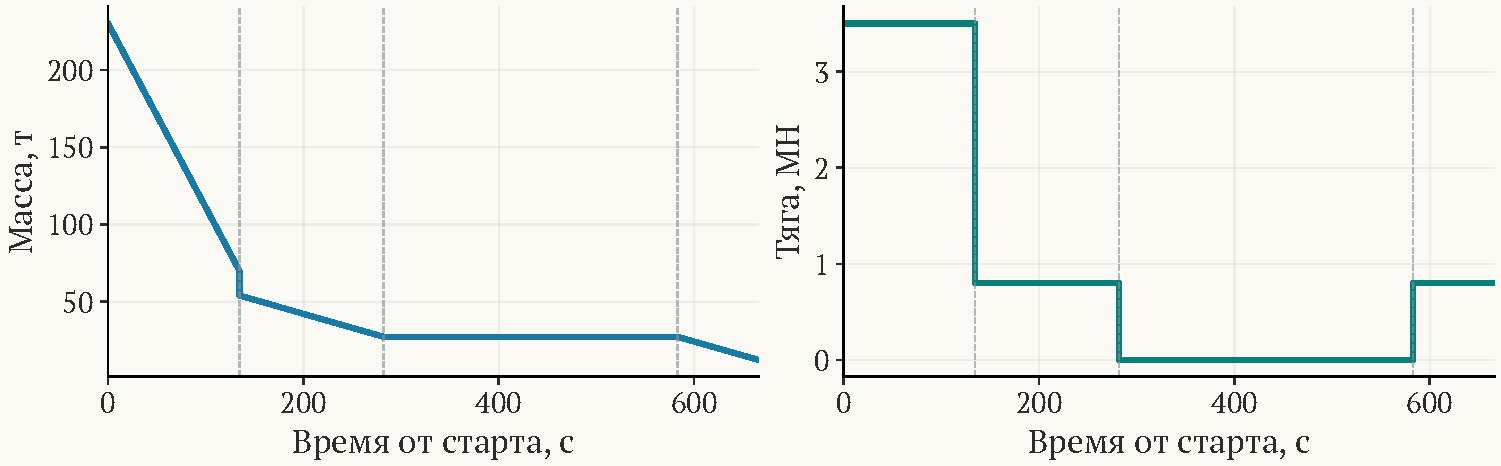
\includegraphics[width=\textwidth,height=44mm,keepaspectratio]{images/ascent-propulsion-slide.pdf}\par}
\justifying
На активных участках масса убывает непрерывно; разделение создаёт её скачок без скачка скорости.
Конечная масса $\AscentFinalMass$ т включает $9$ т сухой ступени и нагрузки; остаток топлива $\AscentReserve$ т.
\end{frame}

\begin{frame}{Тяговая перегрузка}
\relax\derivationmathspacing
{\centering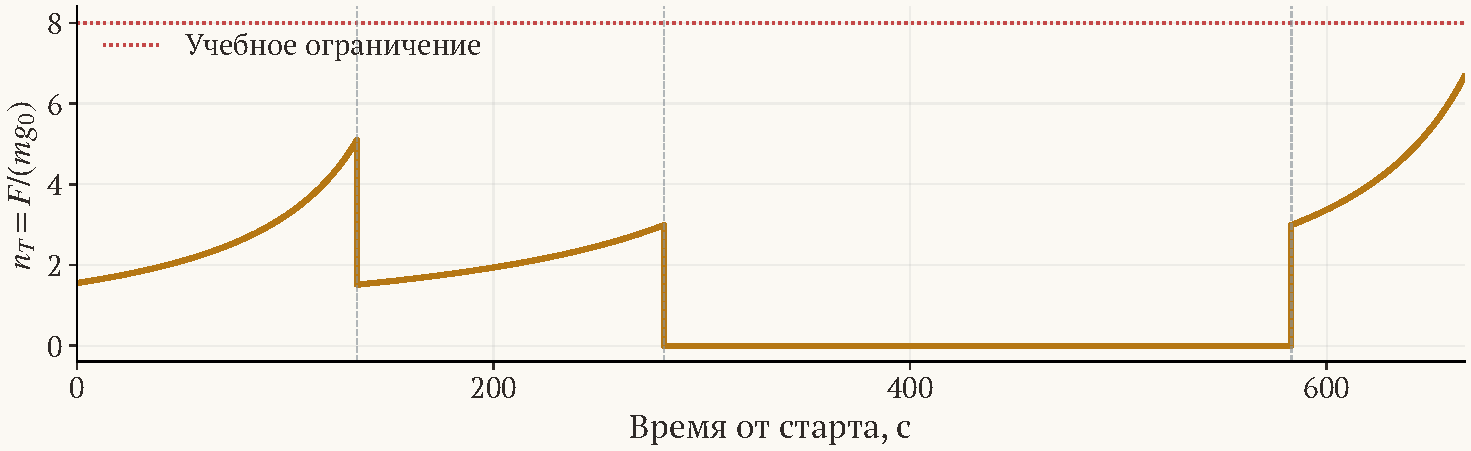
\includegraphics[width=\textwidth,height=43mm,keepaspectratio]{images/ascent-load-slide.pdf}\par}
\justifying
При постоянной тяге уменьшение массы увеличивает $n_T=F/(mg_0)$.
Максимум на сетке с шагом не более $1$ с равен $\AscentMaxLoad$ при учебном пределе $n_T\le8$.
Отдельный расчёт прочности здесь не выполняется.
\end{frame}

\begin{frame}{Аэродинамические нагрузки}
\relax\derivationmathspacing
{\centering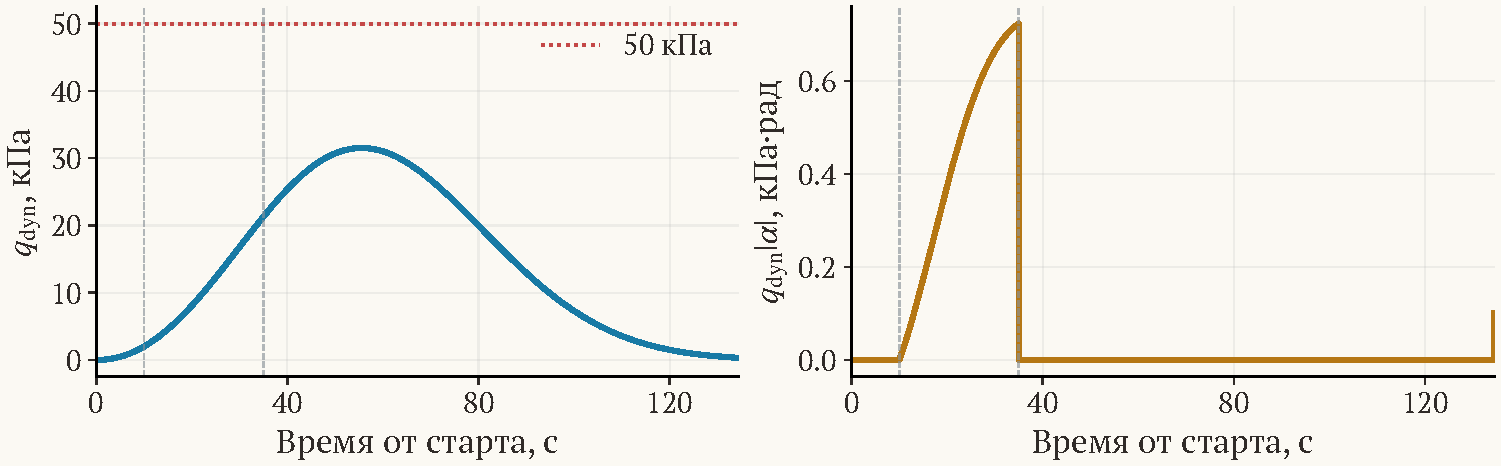
\includegraphics[width=\textwidth,height=43mm,keepaspectratio]{images/ascent-aeroloads-slide.pdf}\par}
\justifying
В начальном развороте $|\alpha|_{\max}\simeq2{,}68^\circ$;
максимумы $q_{\mathrm{dyn}}$ и $q_{\mathrm{dyn}}|\alpha|$ равны $\AscentMaxQ$ кПа и $\AscentMaxQAlpha$ кПа$\cdot$рад.
При тяге вдоль скорости $\alpha=0$.
На верхнем участке рассогласование достигает $20{,}4^\circ$,
но напор не превышает $0{,}323$ кПа.
\end{frame}

\begin{frame}{Скоростной баланс}
\relax\derivationmathspacing
{\centering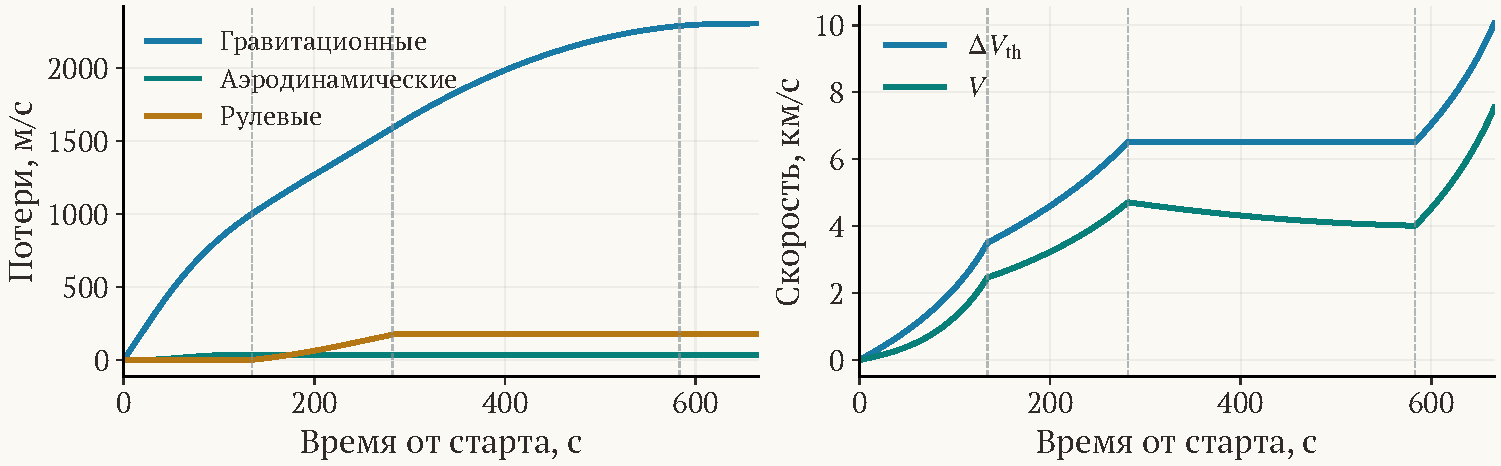
\includegraphics[width=\textwidth,height=39mm,keepaspectratio]{images/ascent-losses-slide.pdf}\par}
{\eqcompact\derivationmathspacing
\[
 \underbrace{10{,}047968}_{\Delta V_{\mathrm{th}}}
 -\underbrace{2{,}303188}_{\Delta V_g}
 -\underbrace{0{,}036440}_{\Delta V_D}
 -\underbrace{0{,}177407}_{\Delta V_{\mathrm{steer}}}
 =7{,}530933\ \text{км/с}.
\]
}
\justifying
На пассивном подъёме характеристическая скорость постоянна, а гравитационный интеграл растёт.
Рулевые потери накапливаются прежде всего при $\theta=45^\circ$.
\end{frame}

\begin{frame}{Влияние начального разворота}
\relax\derivationmathspacing
{\centering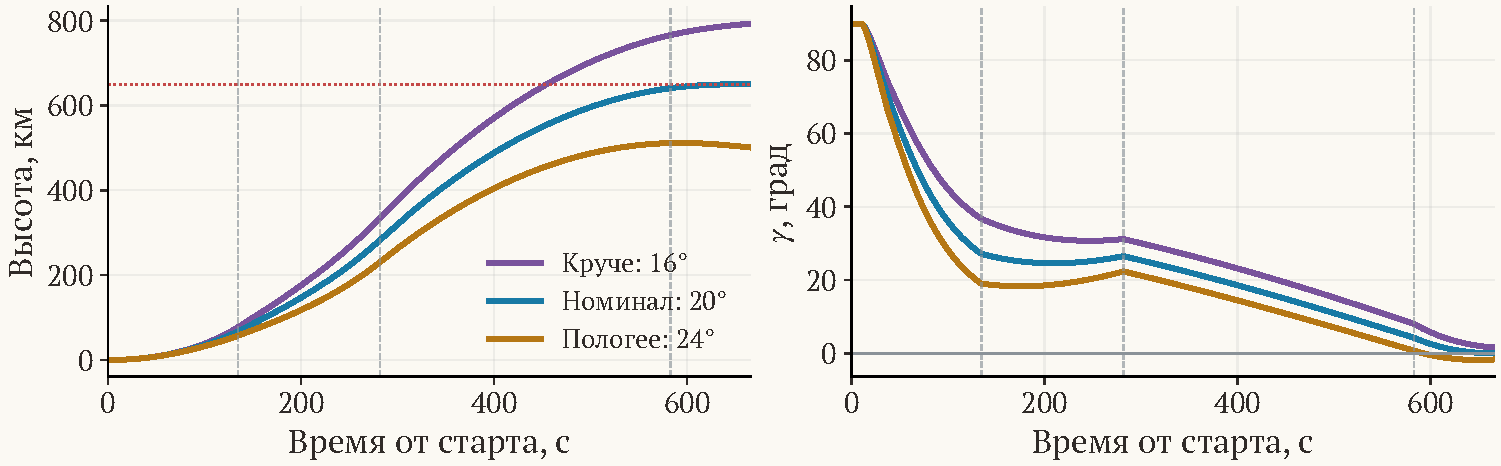
\includegraphics[width=\textwidth,height=39mm,keepaspectratio]{images/ascent-program-comparison-slide.pdf}\par}
\justifying
При тех же длительностях разворот $16^\circ$ даёт высоту $793$ км, но перигей около $-126$ км.
Разворот $24^\circ$ даёт высоту $501$ км и апсиды $447$, $1326$ км.
Расход одинаков; соседние программы повторно не пристреливались.
\end{frame}

\begin{frame}{Результат расчётного примера}
\relax\derivationmathspacing
\begin{columns}[T,onlytextwidth]
\begin{column}{.48\textwidth}
\begin{block}{Конечное состояние}
\begin{itemize}
\setlength{\itemsep}{4pt}
\item Круговая орбита высотой $650$ км.
\item $V_r(t_f)=0$, $V_t(t_f)=V_*$.
\item $t_f=\AscentFinalTime$ с.
\item Конечная масса $\AscentFinalMass$ т; остаток топлива $\AscentReserve$ т.
\end{itemize}
\end{block}
\end{column}
\begin{column}{.49\textwidth}
\begin{block}{Проверки после пристрелки}
\begin{itemize}
\setlength{\itemsep}{4pt}
\item $\norm{\vect{\mathcal R}}_2<10^{-11}$.
\item Напор $\AscentMaxQ<50$ кПа.
\item Перегрузка $\AscentMaxLoad<8$.
\item Повторное интегрирование с более строгими допусками; массовый и скоростной балансы.
\end{itemize}
\end{block}
\end{column}
\end{columns}
\smallskip
\justifying
Пристрелка обеспечила конечные условия и выбранные проверки нагрузок.
Расход топлива не минимизировался, полезная нагрузка не максимизировалась.
\end{frame}


\begin{frame}{Литература}
\relax
\begin{enumerate}
\setlength{\itemsep}{8pt}
 \item Teofilatto P. \textit{Trajectories of Launch and Reentry Systems}.
 Springer, 2025. Разд. 1.2, 1.8--1.9, 2.2--2.7, 3.2--3.4.
 \href{https://doi.org/10.1007/978-3-031-75760-0}{DOI: 10.1007/978-3-031-75760-0}.
 Ступени, аэродинамика, геометрия запуска, атмосферное движение,
 потери, пассивные участки и довыведение.
 \item NASA Glenn Research Center.
 \href{https://www1.grc.nasa.gov/beginners-guide-to-aeronautics/ideal-rocket-equation/}{\textit{Ideal Rocket Equation}};
 \href{https://www1.grc.nasa.gov/beginners-guide-to-aeronautics/dynamic-pressure-2/}{\textit{Dynamic Pressure}}.
 Определения характеристической скорости и скоростного напора.
\end{enumerate}
\end{frame}

\end{document}
